\chapter{BỘ DỮ LIỆU}

\section{Giới Thiệu và Thu Thập}

Nghiên cứu này sử dụng tập dữ liệu tổng hợp từ bốn bộ dữ liệu công khai trên nền tảng Kaggle, mỗi bộ đại diện cho một phương pháp tổng hợp khuôn mặt bằng AI khác nhau. Sự đa dạng về nguồn gốc và phương pháp sinh ảnh là yếu tố then chốt để đảm bảo khả năng tổng quát hóa của mô hình.

\subsection{Mô Tả Các Nguồn Dữ Liệu}

Bảng~\ref{tab:datasets} trình bày thông tin chi tiết của bốn bộ dữ liệu được sử dụng.

\begin{table}[H]
  \centering
  \caption{Các bộ dữ liệu sử dụng trong nghiên cứu}
  \label{tab:datasets}
  \begin{tabularx}{\linewidth}{lXll}
    \toprule
    \textbf{Bộ dữ liệu} & \textbf{Đường dẫn (\texttt{data/raw/})} & \textbf{Quy mô} & \textbf{Phương pháp sinh} \\
    \midrule
    140k-StyleGAN  & \texttt{140k-real-and-fake-faces/} & 70k thật + 70k giả & StyleGAN2 \\
    Deepfake-Real  & \texttt{deepfake-and-real-images/}  & 105.447 ảnh $256{\times}256$ & Manipulation-based \\
    Hard-FakeReal  & \texttt{hardfakevsrealfaces/}        & 1.289 ảnh & GAN bậc cao \\
    ciplab         & \texttt{real-and-fake-face-detection/} & 2.041 ảnh & Nhiều phương pháp GAN \\
    \bottomrule
  \end{tabularx}
\end{table}

\subsection{Quy Trình Hợp Nhất và Tiền Xử Lý}

Quá trình xây dựng tập dữ liệu thống nhất được thực hiện qua notebook \texttt{01\_dataset\_preparation.ipynb}:

\begin{enumerate}
  \item \textbf{Suy ra nhãn từ cấu trúc thư mục:} Nhãn \texttt{Real} (thật) gán cho thư mục \texttt{real}, \texttt{Real}, \texttt{training\_real}; nhãn \texttt{Fake} (giả) gán cho \texttt{fake}, \texttt{Fake}, \texttt{training\_fake}.
  \item \textbf{Loại bỏ ảnh trùng lặp bằng MD5:} Mỗi file ảnh được tính giá trị băm MD5 --- hai ảnh có cùng giá trị MD5 được xem là giống nhau và chỉ giữ lại một bản. Bước này ngăn chặn nguy cơ rò rỉ dữ liệu (data leakage).
  \item \textbf{Phân chia dữ liệu có tầng (stratified split):} Tỷ lệ \textbf{70\% huấn luyện / 15\% kiểm định / 15\% kiểm tra}, \texttt{random\_state=42}. Kết quả lưu vào \texttt{data/splits/train.csv}, \texttt{val.csv}, \texttt{test.csv}.
\end{enumerate}

Schema CSV: mỗi hàng gồm \texttt{image\_path} (đường dẫn tuyệt đối) và \texttt{label} (chuỗi: \texttt{Real} = thật, \texttt{Fake} = giả; được ánh xạ sang $0$/$1$ trong \texttt{FaceDataset}).

Hình~\ref{fig:data_pipeline} trực quan hóa toàn bộ quy trình trên dưới dạng sơ đồ luồng từ bốn nguồn dữ liệu thô đến bộ ba tập huấn luyện/kiểm định/kiểm tra sẵn sàng cho mô hình.

\begin{figure}[H]
  \centering
  \begin{tikzpicture}[
    node distance=0.6cm and 0.3cm,
    proc/.style  = {rectangle, rounded corners=3pt, draw=uitblue, fill=uitblue!8,
                    minimum width=8.6cm, minimum height=0.88cm, align=center, font=\small},
    src/.style   = {rectangle, rounded corners=3pt, draw=gray!60, fill=gray!8,
                    minimum width=1.85cm, minimum height=0.75cm, align=center, font=\footnotesize},
    csv/.style   = {rectangle, rounded corners=3pt, draw=green!60!black, fill=green!7,
                    minimum width=2.45cm, minimum height=0.88cm, align=center, font=\footnotesize},
    arr/.style   = {-Stealth, semithick, gray!70}
  ]
    \node[src] (sA) {140k\\StyleGAN};
    \node[src, right=0.35cm of sA] (sB) {Deepfake\\Real};
    \node[src, right=0.35cm of sB] (sC) {Hard\\FakeReal};
    \node[src, right=0.35cm of sC] (sD) {ciplab};

    \node[proc, below=0.9cm of sB, xshift=0.78cm] (p1)
      {Bước 1 --- Suy nhãn từ tên thư mục \quad Real=0, Fake=1};
    \node[proc, below=0.55cm of p1] (p2)
      {Bước 2 --- MD5 Deduplication $\;\longrightarrow\;$ \textbf{316.530 ảnh}};
    \node[proc, below=0.55cm of p2] (p3)
      {Bước 3 --- Stratified Split 70 / 15 / 15 \quad (\texttt{random\_state=42})};

    \node[csv, below=0.85cm of p3, xshift=-3.1cm] (oTr)
      {\texttt{train.csv} / 221.571};
    \node[csv, below=0.85cm of p3]  (oV)
      {\texttt{val.csv} / 47.479};
    \node[csv, below=0.85cm of p3, xshift=3.1cm] (oTe)
      {\texttt{test.csv} / 47.480};

    \node[proc, below=0.85cm of oV] (p4)
      {Bước 4 --- FaceDataset + DataLoader \quad (batch\_size=128, augmentation train only)};

    \draw[arr] (sA.south) -- ++(0,-0.38) -| (p1.north);
    \draw[arr] (sB.south) -- ++(0,-0.38) -| (p1.north);
    \draw[arr] (sC.south) -- ++(0,-0.38) -| (p1.north);
    \draw[arr] (sD.south) -- ++(0,-0.38) -| (p1.north);

    \draw[arr] (p1) -- (p2);
    \draw[arr] (p2) -- (p3);

    \draw[arr] (p3.south) -- ++(0,-0.38) -| (oTr.north);
    \draw[arr] (p3.south) -- ++(0,-0.38) -- (oV.north);
    \draw[arr] (p3.south) -- ++(0,-0.38) -| (oTe.north);

    \draw[arr] (oTr.south) -- ++(0,-0.38) -| (p4.north);
    \draw[arr] (oV.south)  -- (p4.north);
    \draw[arr] (oTe.south) -- ++(0,-0.38) -| (p4.north);
  \end{tikzpicture}
  \caption{Quy trình hợp nhất và chuẩn bị bộ dữ liệu từ bốn nguồn Kaggle}
  \label{fig:data_pipeline}
\end{figure}

\subsection{Thống Kê Tập Dữ Liệu Sau Hợp Nhất}

\begin{table}[H]
  \centering
  \caption{Thống kê phân bố dữ liệu sau split}
  \label{tab:splits}
  \begin{tabular}{lrrrr}
    \toprule
    \textbf{Tập} & \textbf{Tổng ảnh} & \textbf{Thật (Real)} & \textbf{Giả (Fake)} & \textbf{Tỷ lệ thật} \\
    \midrule
    Huấn luyện (Train) & 221.571 & 104.819 & 116.752 & 47,3\% \\
    Kiểm định (Val)    &  47.479 &  22.461 &  25.018 & 47,3\% \\
    Kiểm tra (Test)    &  47.480 &  22.461 &  25.019 & 47,3\% \\
    \midrule
    \textbf{Tổng cộng} & \textbf{316.530} & \textbf{149.741} & \textbf{166.789} & \textbf{47,3\%} \\
    \bottomrule
  \end{tabular}
\end{table}

Mức mất cân bằng lớp nhẹ ($\approx 5{,}4$ điểm phần trăm) không đòi hỏi điều chỉnh trọng số lớp trong hàm mất mát.

\section{Quy Trình Khai Phá Dữ Liệu (EDA)}

Phân tích EDA được thực hiện tại notebook \texttt{02\_eda.ipynb} vào ngày 17/05/2026.

\subsection{Phân Bố Lớp Theo Nguồn Dữ Liệu}

\begin{figure}[H]
  \centering
  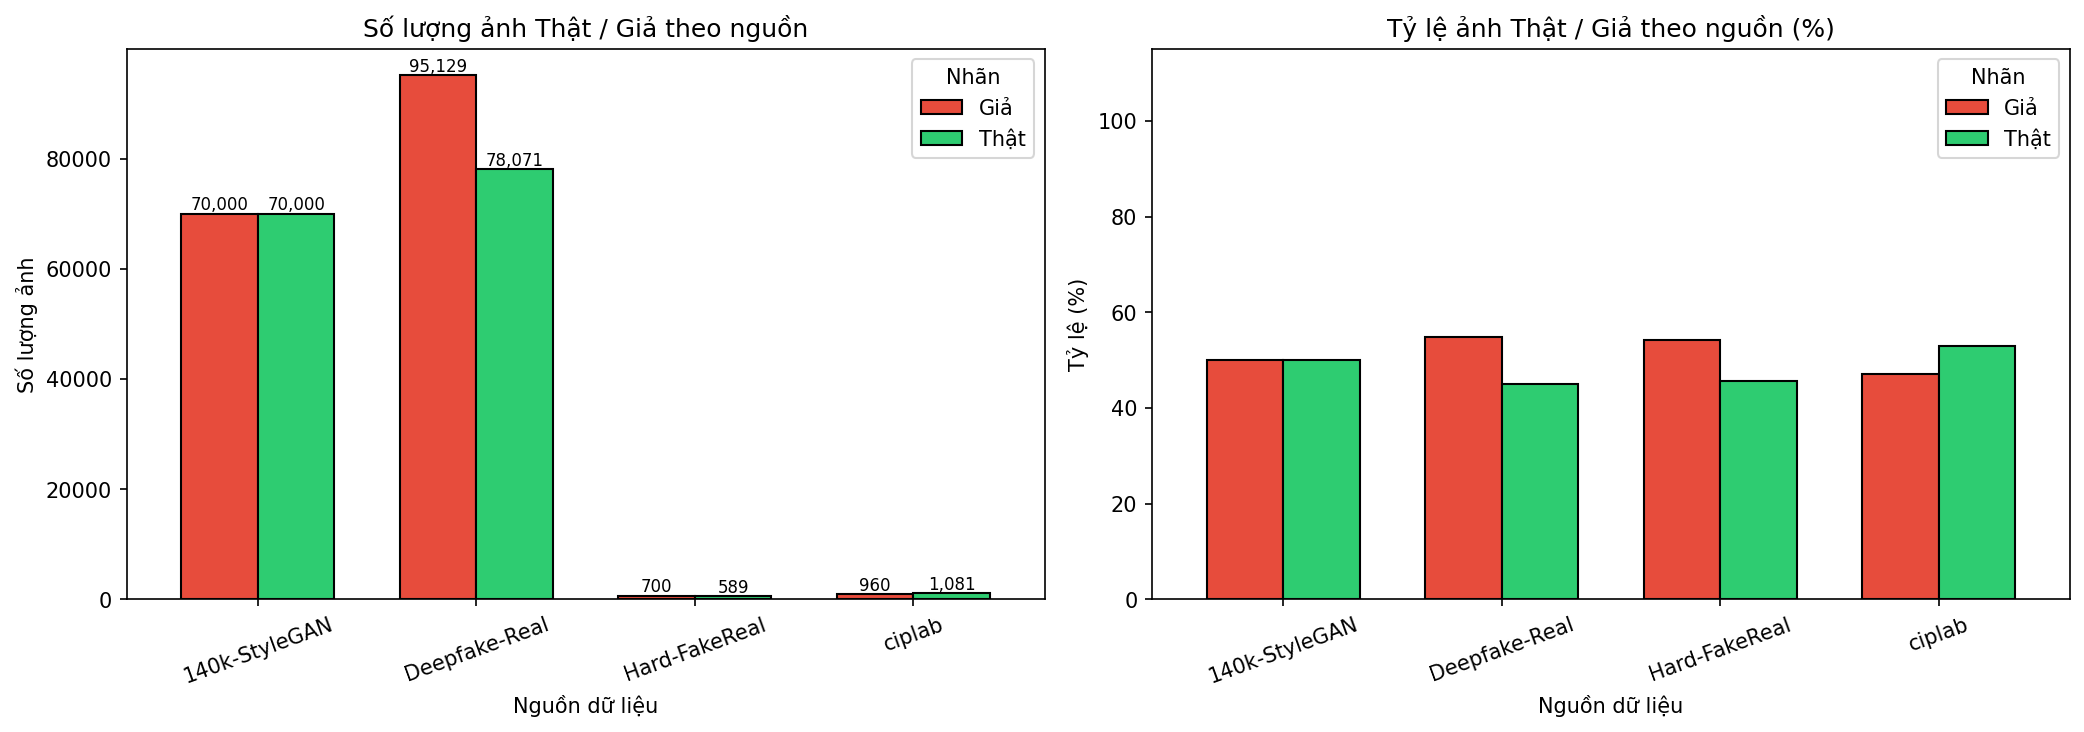
\includegraphics[width=0.85\linewidth]{eda/assets/eda_class_distribution.png}
  \caption{Phân bố số lượng ảnh thật và giả theo từng nguồn dữ liệu}
  \label{fig:class_dist}
\end{figure}

Bộ 140k-StyleGAN có phân bố hoàn toàn cân bằng (70.000 thật --- 70.000 giả) và chiếm khoảng 44\% tổng thể. Ưu thế quy mô của bộ này yêu cầu lưu ý: nếu không có chiến lược lấy mẫu phù hợp, mô hình có nguy cơ chủ yếu học đặc trưng của ảnh StyleGAN2.

\begin{table}[H]
  \centering
  \caption{Phân bố dữ liệu theo nguồn}
  \label{tab:source_dist}
  \begin{tabular}{lrrrr}
    \toprule
    \textbf{Nguồn} & \textbf{Tổng} & \textbf{Thật} & \textbf{Giả} & \textbf{T/G Ratio} \\
    \midrule
    140k-StyleGAN & 140.000 & 70.000 & 70.000 & 1,000 \\
    Deepfake-Real & 105.447 & 29.959 & 75.488 & 0,397 \\
    Hard-FakeReal & 1.289   &    589 &    700 & 0,841 \\
    ciplab        & 2.041   &  1.081 &    960 & 1,126 \\
    \midrule
    \textbf{Tổng cộng} & \textbf{248.777} & \textbf{101.629} & \textbf{147.148} & \textbf{0,691} \\
    \bottomrule
  \end{tabular}
\end{table}

\subsection{Phân Bố Độ Phân Giải}

\begin{figure}[H]
  \centering
  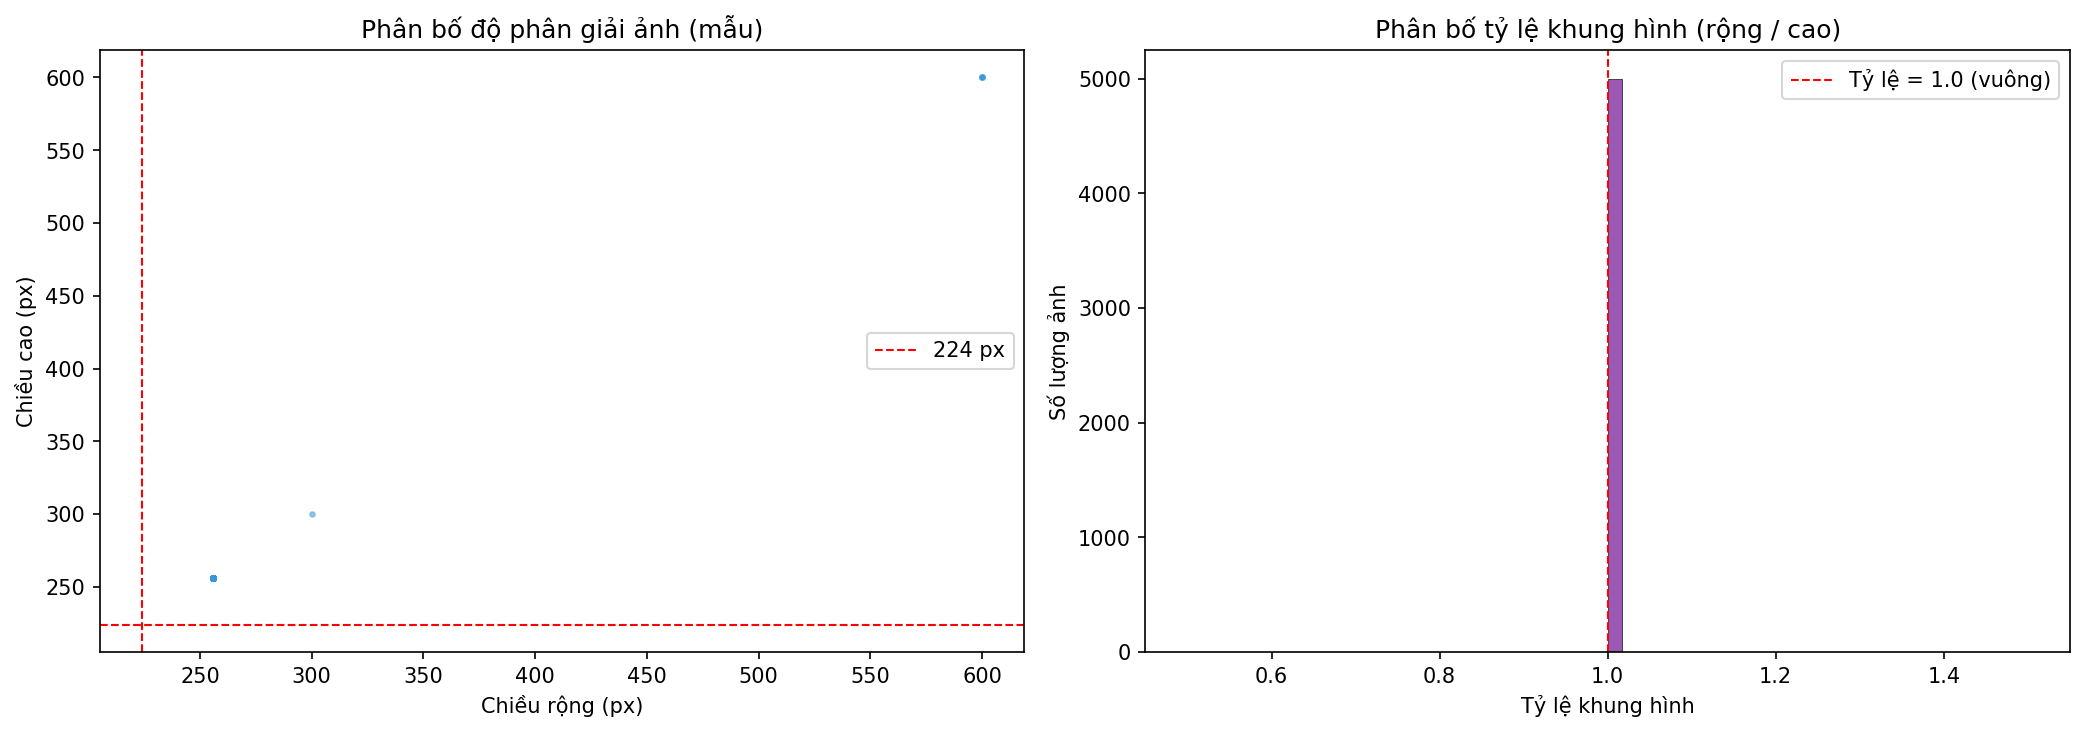
\includegraphics[width=0.85\linewidth]{eda/assets/eda_resolution.png}
  \caption{Phân bố độ phân giải và tỷ lệ khung hình của tập dữ liệu}
  \label{fig:resolution}
\end{figure}

Ảnh 140k-StyleGAN đã ở kích thước $224 \times 224$ --- phù hợp trực tiếp với EfficientNet-B0. Ảnh Deepfake-Real có kích thước gốc $256 \times 256$; resize về $224 \times 224$ chỉ mất tối thiểu thông tin. Hầu hết ảnh có tỷ lệ khung hình $\approx 1{:}1$ (vuông) --- resize không gây biến dạng hình học đáng kể.

\subsection{Phân Tích Thuộc Tính Pixel}

\begin{figure}[H]
  \centering
  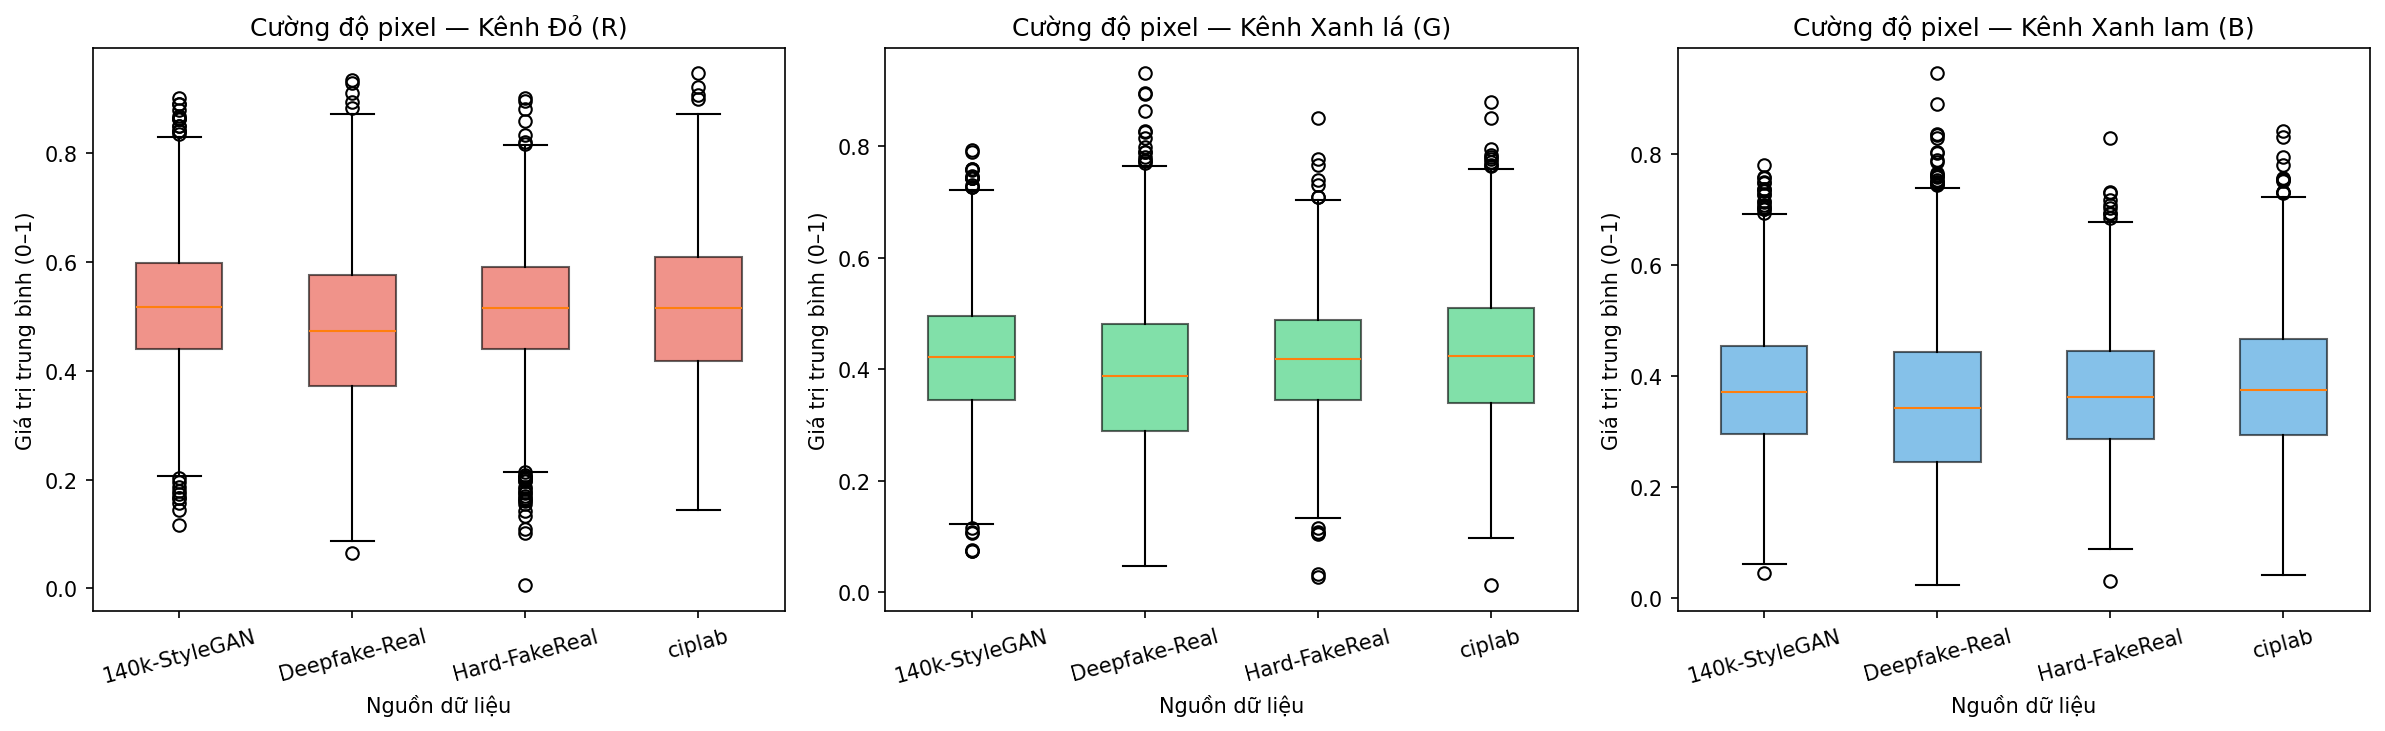
\includegraphics[width=0.85\linewidth]{eda/assets/eda_pixel_stats.png}
  \caption{Thống kê cường độ pixel R/G/B theo nguồn dữ liệu}
  \label{fig:pixel_stats}
\end{figure}

Phân bố pixel tương đối đồng nhất giữa bốn nguồn dữ liệu trong cùng kênh màu --- không có domain shift màu sắc cực đoan. Kênh R có xu hướng cao hơn kênh B, phù hợp với tông da người. Điều này xác nhận rằng chuẩn hóa ImageNet là lựa chọn phù hợp và không cần xử lý màu bổ sung.

\subsection{Phân Tích Mẫu Đại Diện}

\begin{figure}[H]
  \centering
  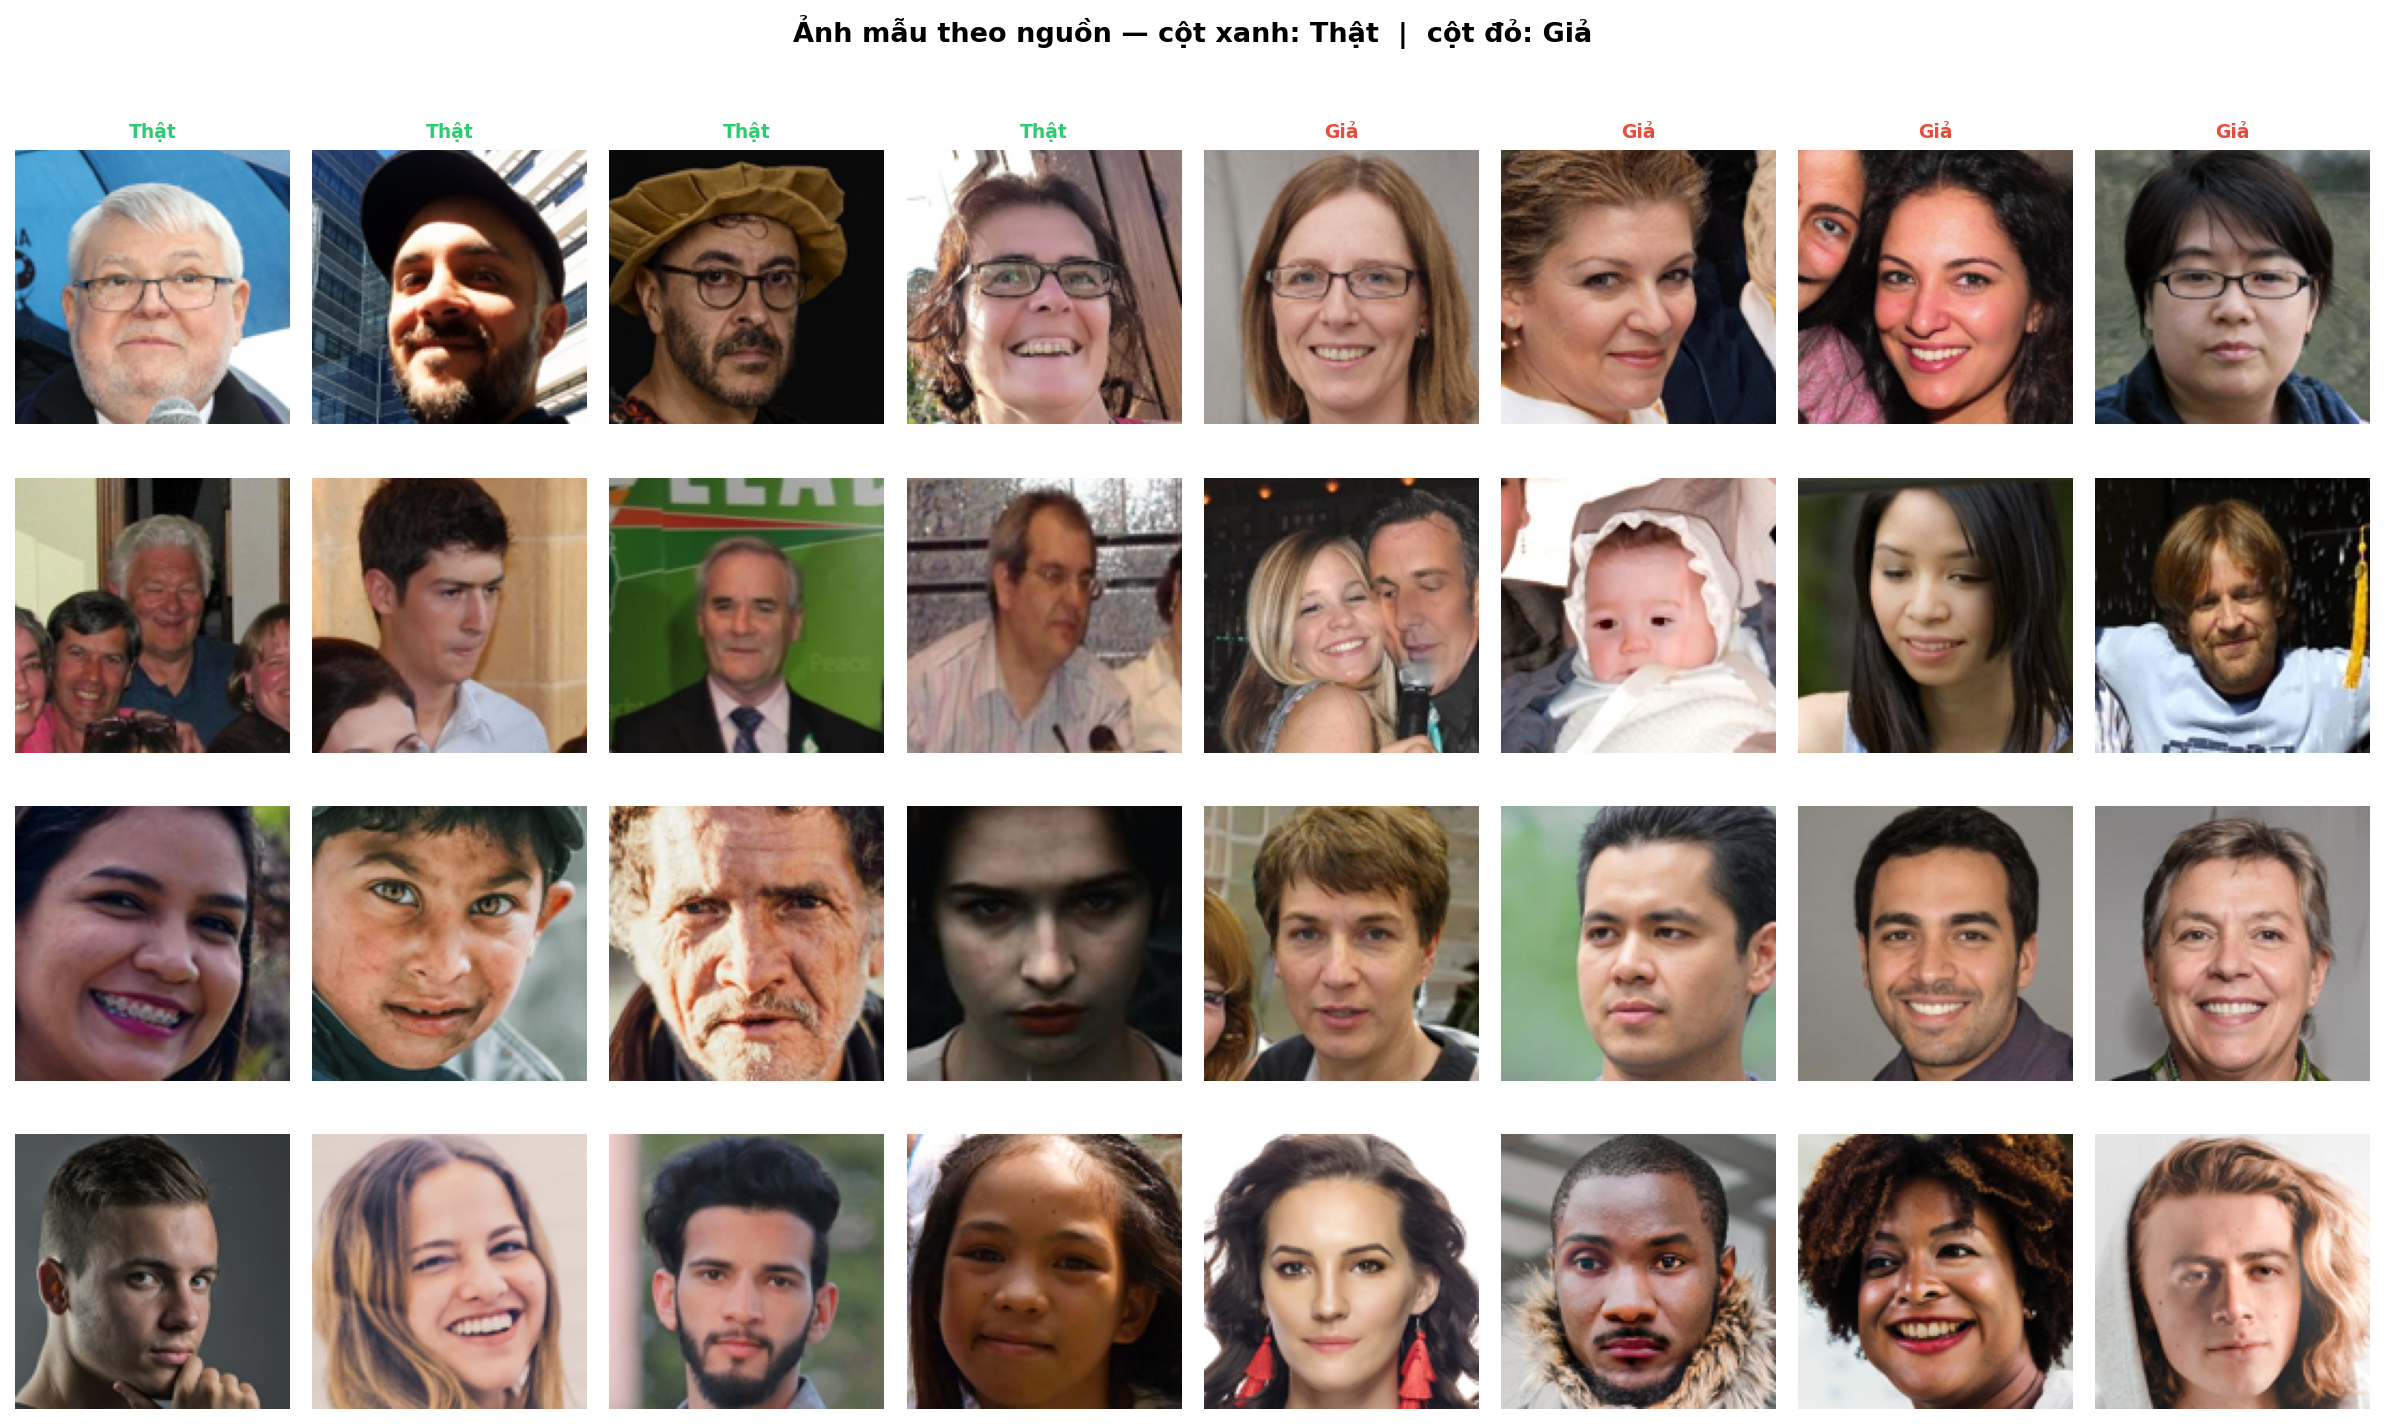
\includegraphics[width=\linewidth]{eda/assets/eda_sample_grid.png}
  \caption{Lưới ảnh mẫu: ảnh thật (viền xanh lá) và ảnh giả (viền đỏ) theo từng nguồn}
  \label{fig:sample_grid}
\end{figure}

Quan sát trực quan cho thấy sự khác biệt rõ rệt về đặc điểm artifact giữa các nguồn: StyleGAN2 để lại artifact ở vùng tai và tóc; deepfake manipulation-based có vùng biên khuôn mặt không tự nhiên; Hard-FakeReal được thiết kế để tối đa hóa độ khó phân biệt.

\subsection{Phân Tích Phổ Tần Số (FFT)}

\begin{figure}[H]
  \centering
  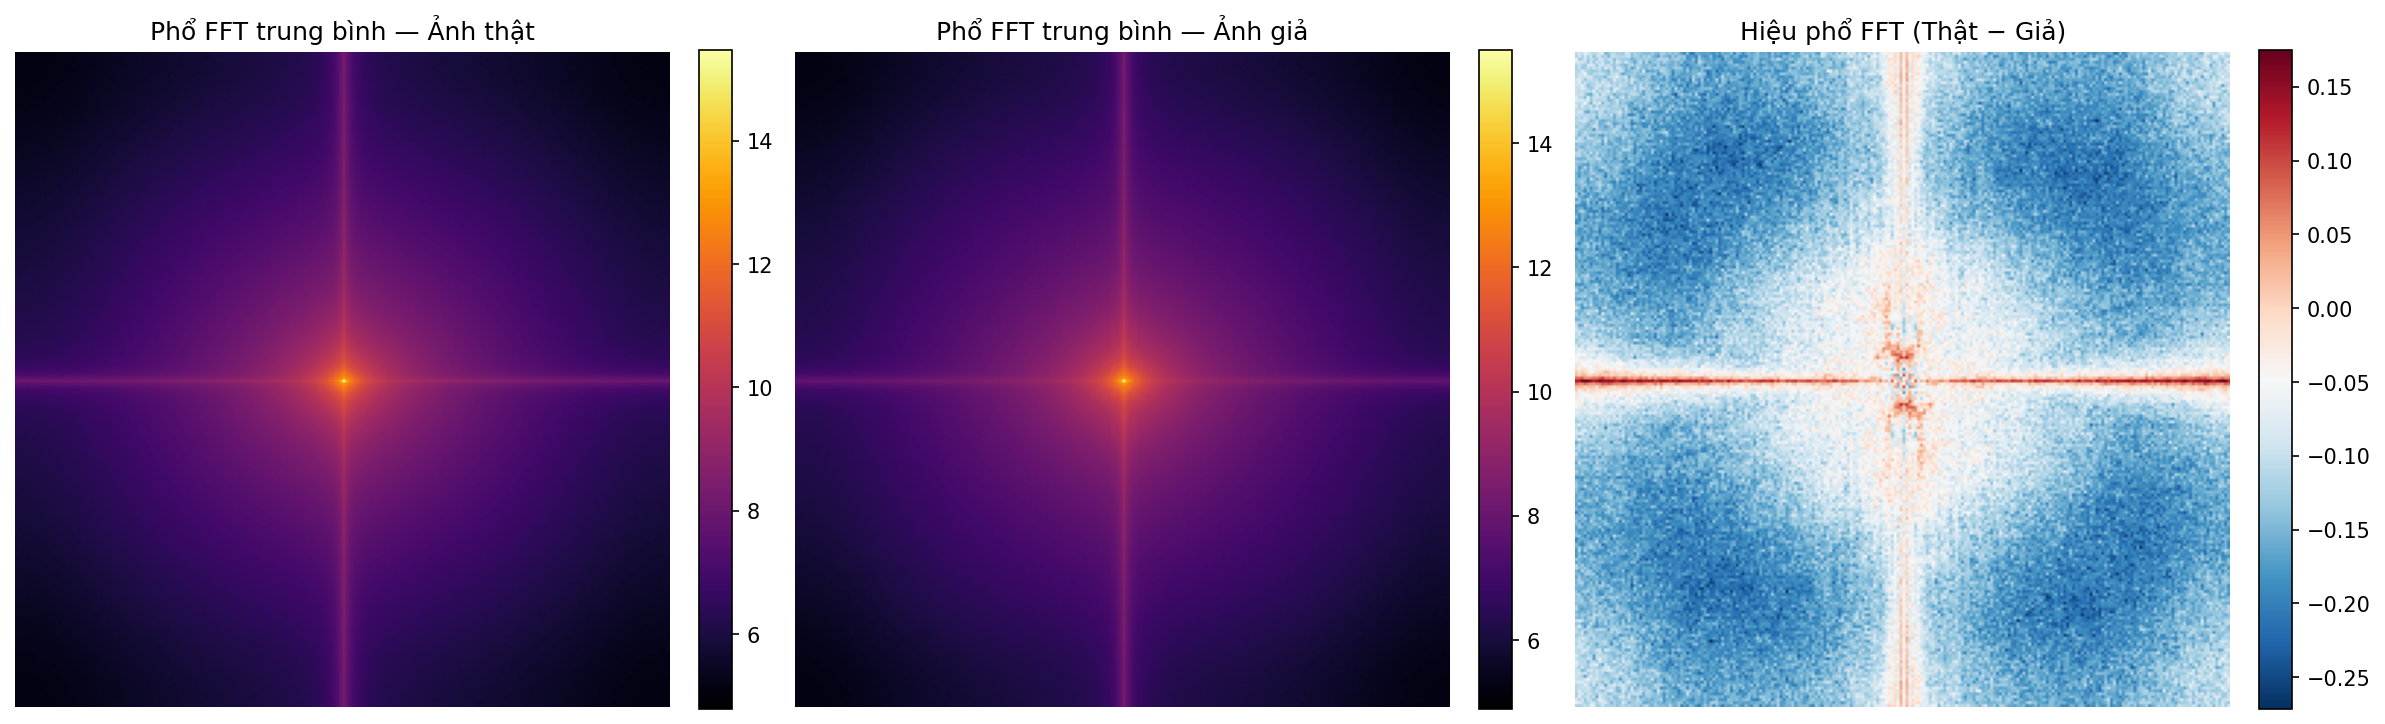
\includegraphics[width=0.85\linewidth]{eda/assets/eda_fft.png}
  \caption{Phân tích phổ FFT: phổ trung bình của ảnh thật (trái), ảnh giả (giữa) và hiệu phổ (phải)}
  \label{fig:fft}
\end{figure}

Phân tích FFT tiết lộ đặc điểm quan trọng: ảnh giả có năng lượng dư thừa ở mức chi tiết nhỏ (tần số cao) --- dấu vết của quá trình AI tạo ảnh. Hiệu phổ (Thật $-$ Giả) cho thấy ảnh giả thiếu sự mịn màng tự nhiên ở mức chi tiết vừa. Đây là cơ sở lý giải tại sao EfficientNet-B0 --- kiến trúc CNN học đặc trưng cục bộ ở nhiều mức độ --- là lựa chọn phù hợp.

\subsection{Kiểm Tra Tính Toàn Vẹn Dữ Liệu}

Kiểm tra chồng lấp giữa ba tập train/val/test bằng phép giao tập hợp đường dẫn ảnh xác nhận:
\begin{itemize}
  \item Train $\cap$ Val: $\emptyset$ (không trùng lặp)
  \item Train $\cap$ Test: $\emptyset$ (không trùng lặp)
  \item Val $\cap$ Test: $\emptyset$ (không trùng lặp)
\end{itemize}
Ba tập hoàn toàn độc lập --- kết quả đánh giá trên tập test là đáng tin cậy và không bị ảnh hưởng bởi rò rỉ dữ liệu.

\section{Nhận Xét Chất Lượng Bộ Dữ Liệu}

\subsection{Kích Thước và Cấu Trúc}

Với tổng cộng \textbf{316.530 ảnh} sau loại bỏ trùng lặp MD5 --- trong đó 221.571 ảnh dùng để huấn luyện --- bộ dữ liệu có quy mô đủ lớn để huấn luyện mô hình deep learning. Mức độ mất cân bằng lớp nhẹ (47,3\% thật --- 52,7\% giả) không đòi hỏi điều chỉnh trọng số lớp: Precision cao (97,73\%) trên tập test bác bỏ giả thuyết mô hình thiên vị về lớp đa số.

\subsection{Thách Thức Kỹ Thuật}

\begin{itemize}
  \item \textbf{Domain shift giữa các nguồn:} Bốn bộ dữ liệu khác nhau về phương pháp sinh ảnh, độ phân giải gốc và đặc điểm artifact. Đây là lý do cốt lõi để thiết kế bài kiểm tra cross-generator.

  \item \textbf{Hard-FakeReal:} Bộ dữ liệu này đặc biệt thách thức do ảnh giả được thiết kế có chủ đích để khó phân biệt --- mô hình cần học đặc trưng tinh vi ở mức pixel.

  \item \textbf{Ưu thế số lượng của 140k-StyleGAN ($\approx 44\%$):} Cần đảm bảo mô hình không học thiên về phong cách ảnh StyleGAN2 mà bỏ qua đặc trưng của các bộ còn lại.
\end{itemize}
